\TODO

\section{Spartan-6 SP605 Evaluation Platform}

The Spartan-6 SP605 Evaluation Platform is essentially a board with the Spartan-6 LX45T FPGA wired to every useful peripheral imaginable.
It has connections for PCI Express\footnote{
        Even though the PCI Express finger has lines for power, they are not connected on the SP605. This means an external power source has to be connected.
    }, ethernet, DVI, USB, flash card, JTAG, LEDs, switches, and more.
However, the only peripherals utilized in this paper are PCI Express, and JTAG.
An overview of the system is shown in \figurename~\ref{fig:sp605}.

\begin{figure}[!ht]
    \centering
    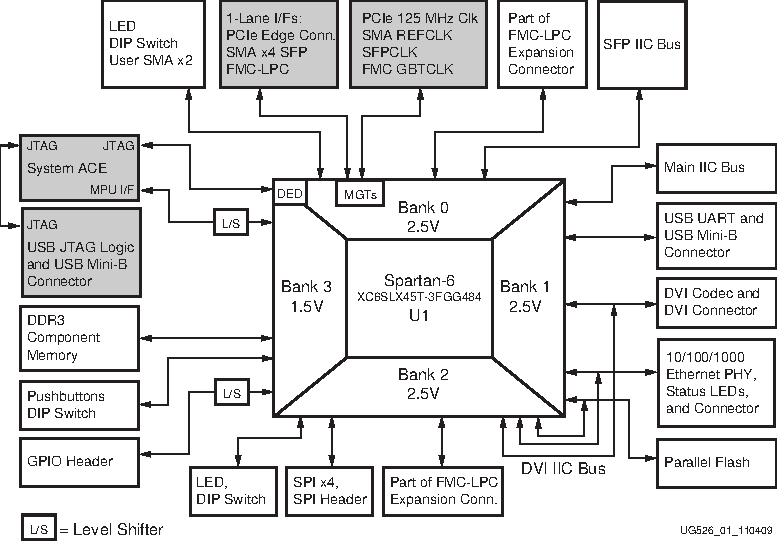
\includegraphics[width=\textwidth]{figures/sp605-modified}
    \caption[SP605]{
        High-level block diagram of the SP605 and its peripherals.
        Peripherals utilized in this paper are highlighted in gray.
        (Modified reprint from \cite{ug526})
    }
    \label{fig:sp605}
\end{figure}

The switch and jumper configurations of the SP605 are set to factory defaults, with the exception of SW1 which is set to 10.

\section{Hardware Setup}

Due to the experimental nature of testing a new hardware platform, two computers were used in this project, as shown in \figurename~\ref{fig:hardware-setup}.
One is the main development workstation, used for coding and synthesis; it has a JTAG connection to the SP605 over USB, which allows it to upload new designs.
The other is the host for the SP605, which is mounted in a PCI Express expansion slot.

\begin{figure}[!ht]
    \centering
    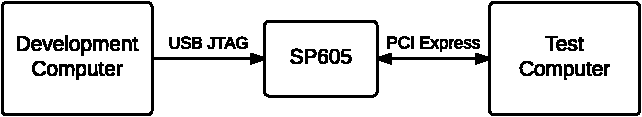
\includegraphics[width=0.70\textwidth]{figures/hardware-setup}
    \caption[Hardware setup]{
        High-level block diagram of the hardware setup.
    }
    \label{fig:hardware-setup}
\end{figure}

The setup allows a new design to be uploaded and tested on the SP605 without disrupting the workflow of the main workstation, due to the power-cycle required to reset the PCI Express connection.

\section{Software Setup}

The operating system on both computers is Linux Mint; version 16 on the development computer and 17 on the test computer.
Linux Mint is currently one of the most popular linux distributions, along with Ubuntu, which it is based upon \cite{distrowatch}.
This means that procedures and software used and created in this paper should work on most systems.
\todo{also Manjaro/Arch}

Xilinx ISE version 13.3 was used for hardware design and synthesis, while ISim was used for simulations.
The third-party USB cable driver from \cite{usbdriver} was used for JTAG, as explained in Section~\ref{sec:challenges}.
The software API was compiled with GCC version 4.8.2.

